\begin{dang}{Tìm các đường tiệm cận qua biểu thức hàm số, bảng biến thiên}
\end{dang}
\begin{vd} Tìm các đường tiệm cận đứng, ngang, xiên (nếu có) của đồ thị hàm số sau
    \begin{listEX}[3]
        \item $y=\dfrac{2x+1}{x+1}$.
        \item $y=\dfrac{x}{2x-1}$.
        \item $y=\dfrac{3-x}{x+1}$.
        \item $y=2x+1+\dfrac{1}{x-3}$
        \item $y=\dfrac{4x^2-3x+10}{x-1}$.
        \item $y=\dfrac{x^2-4x+3}{x^2-1}$.
        \item $y=\dfrac{2x+4}{x^2+x-2}$.
        \item $y=\dfrac{\sqrt{9-x^2}}{x-1}$.
        \item $y=x+\sqrt{x^2-1}$
        %	\item $y=\dfrac{x}{\sqrt{x^2+1}}$.
        %	\item $y=\dfrac{\sqrt{x+25}-5}{x^2+x}$.
    \end{listEX}
    \loigiai{}
\end{vd}
\begin{vd}
    Tìm các đường tiệm cận của đồ thị hàm số $y=f(x)$, biết
    \begin{listEX}[2]
        \item 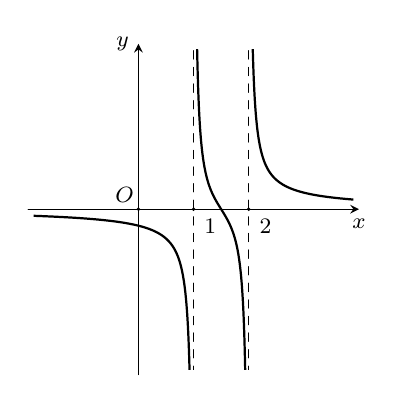
\begin{tikzpicture}[scale=.7,>=stealth, font=\footnotesize, line join=round, line cap=round]
            \def\xmin{-2} \def\xmax{4}
            \def\ymin{-3} \def\ymax{3}
            %\draw[color=gray!50,dashed] (\xmin,\ymin) grid (\xmax,\ymax);
            \draw[->] (\xmin,0)--(\xmax,0) node [below]{$x$};
            \draw[->] (0,\ymin)--(0,\ymax) node [left]{$y$};
            \fill (0,0) circle (1pt) node[shift={(135:2.5mm)}]{$O$};
            %\node at (current bounding box.south) [below=-2pt] {a) $y=\dfrac{2x-3}{5x^{2}-15x+10}$};
            \clip (\xmin+0.1,\ymin+0.1) rectangle (\xmax-0.1,\ymax-0.1);
            \draw[thick,smooth,samples=300,domain=\xmin:0.99] plot(\x,{(2*(\x)-3)/(5*(\x)^2-15*(\x)+10)});
            \draw[thick,smooth,samples=300,domain=1.01:1.99] plot(\x,{(2*(\x)-3)/(5*(\x)^2-15*(\x)+10)});
            \draw[thick,smooth,samples=300,domain=2.01:\xmax] plot(\x,{(2*(\x)-3)/(5*(\x)^2-15*(\x)+10)});
            \draw[dashed] (1,\ymin)--(1,\ymax);
            \draw[dashed] (2,\ymin)--(2,\ymax);
            \foreach \s/\t in {2/-45,1/-45}
            \fill (\s,0) circle (1pt) node[shift={(\t:3mm)}]{$\s$};
        \end{tikzpicture}
        \item \begin{tikzpicture}[scale=.5,>=stealth, font=\footnotesize, line join=round, line cap=round]
            \def\xmin{-4} \def\xmax{4}
            \def\ymin{-3} \def\ymax{5}
            %\draw[color=gray!50,dashed] (\xmin,\ymin) grid (\xmax,\ymax);
            \draw[->] (\xmin,0)--(\xmax,0) node [below]{$x$};
            \draw[->] (0,\ymin)--(0,\ymax) node [right]{$y$};
            \fill (0,0) circle (1pt) node[shift={(-135:2.5mm)}]{$O$};
            %\node at (current bounding box.south) [below=-2pt] {c) $y=\dfrac{16x^{2}-8x}{16x^{2}+1}$};
            \clip (\xmin+0.1,\ymin+0.1) rectangle (\xmax-0.1,\ymax-0.1);
            \draw[thick,smooth,samples=300,domain=\xmin:\xmax] plot(\x,{(16*(\x)^2-8*(\x))/(16*(\x)^2+1)});
            \draw[dashed](\xmin,1)--(\xmax,1);
            \foreach \p/\r in {1/45}
            \fill (0,\p) circle (1pt) node[shift={(\r:3mm)}]{$\p$};
        \end{tikzpicture}
        \item 	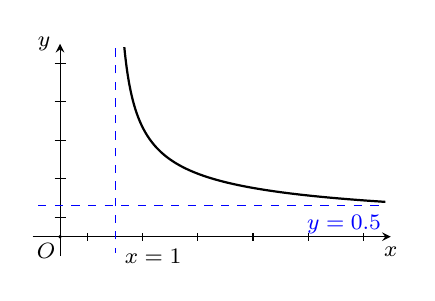
\begin{tikzpicture}[scale=.7,>=stealth, font=\footnotesize, y=.7cm]
            \def\xmin{-.5} \def\xmax{6}
            \def\ymin{-.5} \def\ymax{5}
            \draw[->] (\xmin,0)--(\xmax,0) node [below]{$x$};
            \draw[->] (0,\ymin)--(0,\ymax) node [left]{$y$};
            \fill (0,0) circle (1pt) node[shift={(-135:2.5mm)}]{$O$};
            \node at (1,-.5)[right]{$x=1$};
            \clip (\xmin+0.1,\ymin+0.1) rectangle (\xmax-0.1,\ymax-0.1);
            \draw[smooth,thick,samples=300,domain=(1.01:\xmax)] plot(\x,{2/sqrt(\x-1)});
            \draw[blue,dashed] (1,\ymin)--(1,\ymax);
            \draw[blue,dashed] (-1,.8)--(6,.8)node[below left]{$y=0.5$};
            \foreach \x in {\xmin,...,\xmax}
            \draw (\x,-0.1)--(\x,0.1);
            \foreach \y in {\ymin,...,\ymax}
            \draw (-0.1,\y)--(0.1,\y);
        \end{tikzpicture}
        \item 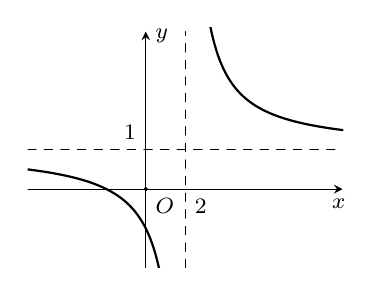
\begin{tikzpicture}[scale=0.5, font=\footnotesize, line join=round, line cap=round, >=stealth]
            \clip(-3,-2) rectangle (5.1,4.1);
            \draw[->] (-3,0) -- (5,0);\draw (4.9,0) node[below] { $x$};
            \draw[->] (0,-2) -- (0,4);\draw (0,3.9) node[right] { $y$};
            \draw[fill=black] (0,0) node[below right]{$O$} circle (1pt);
            \draw (1,0) node[below right]{$2$};
            \draw (0,1) node[above left]{$1$};
            \draw[thick] plot[domain=-3:0.5,samples=100] (\x, {(1 + \x)/(\x - 1)});
            \draw[thick] plot[domain= 1.5:5,samples=100] (\x, {(1 + \x)/(\x - 1)});
            \draw [-,dashed] (-3,1)--(5,1); %TCN
            \draw [-,dashed] (1,-2)--(1,4); %TCĐ
            \draw[fill=black] (0,0) circle(1pt);
        \end{tikzpicture}
        \item 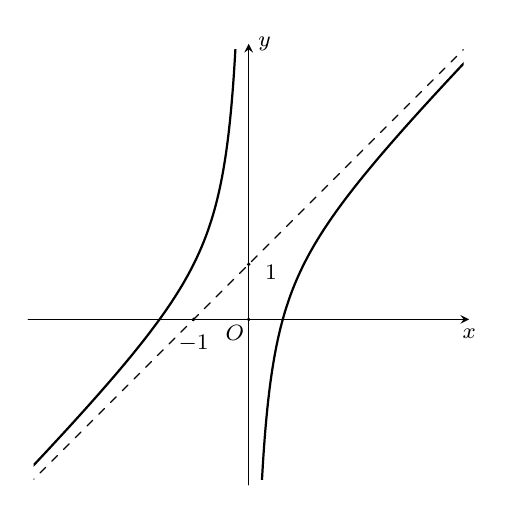
\begin{tikzpicture}[scale=.7,>=stealth, font=\footnotesize, line join=round, line cap=round]
            \def\xmin{-4} \def\xmax{4}
            \def\ymin{-3} \def\ymax{5}
            %\draw[color=gray!50,dashed] (\xmin,\ymin) grid (\xmax,\ymax);
            \draw[->] (\xmin,0)--(\xmax,0) node [below]{$x$};
            \draw[->] (0,\ymin)--(0,\ymax) node [right]{$y$};
            \fill (0,0) circle (1pt) node[shift={(-135:2.5mm)}]{$O$};
            %\node at (current bounding box.south) [below=-2pt] {b) $y=\dfrac{x^{2}+x-1}{x}$};
            \clip (\xmin+0.1,\ymin+0.1) rectangle (\xmax-0.1,\ymax-0.1);
            \draw[thick,smooth,samples=300,domain=\xmin:-0.01] plot(\x,{((\x)^2+(\x)-1)/(\x)});
            \draw[thick,smooth,samples=300,domain=0.01:\xmax] plot(\x,{((\x)^2+(\x)-1)/(\x)});
            \draw[dashed,smooth,samples=300,domain=\xmin:\xmax] plot(\x,{(\x)+1});
            \foreach \s/\t in {-1/-90}
            \fill (\s,0) circle (1pt) node[shift={(\t:3mm)}]{$\s$};
            \foreach \p/\r in {1/-20}
            \fill (0,\p) circle (1pt) node[shift={(\r:3mm)}]{$\p$};
        \end{tikzpicture}
        \item 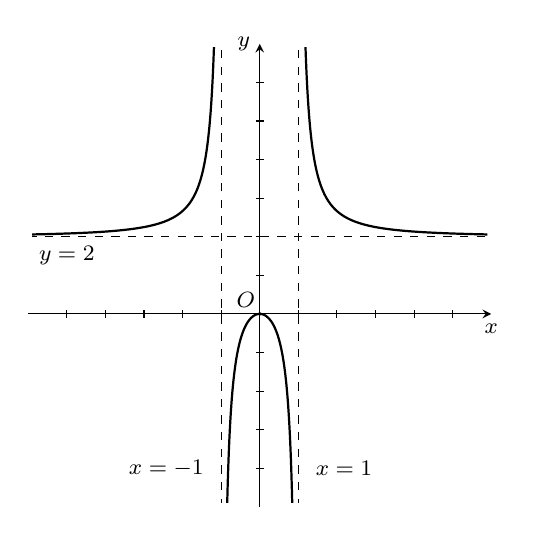
\begin{tikzpicture}[scale=.7,>=stealth, font=\footnotesize,x=.7cm,y=.7cm]
            \def\xmin{-6} \def\xmax{6}
            \def\ymin{-5} \def\ymax{7}
            %\draw[color=gray!50,dashed] (\xmin,\ymin) grid (\xmax,\ymax);
            \draw[->] (\xmin,0)--(\xmax,0) node [below]{$x$};
            \draw[->] (0,\ymin)--(0,\ymax) node [left]{$y$};
            \fill (0,0) circle (1pt) node[shift={(135:2.5mm)}]{$O$};
            \clip (\xmin+0.1,\ymin+0.1) rectangle (\xmax-0.1,\ymax-0.1);
            \draw[smooth,thick,samples=300,domain=(\xmin:-1.01)] plot(\x,{(2*(\x)^2)/((\x)^2-1)});
            \draw[smooth,thick,samples=300,domain=(-0.9:0.9)] plot(\x,{(2*(\x)^2)/((\x)^2-1)});
            \draw[smooth,thick,samples=300,domain=(1.1:\xmax)] plot(\x,{(2*(\x)^2)/((\x)^2-1)});
            \draw[dashed] (\xmin,2)--(\xmax,2);
            \draw[dashed] (-1,\ymin)--(-1,\ymax);
            \draw[dashed] (1,\ymin)--(1,\ymax);
            \foreach \x in {\xmin,...,\xmax}
            \draw (\x,-0.1)--(\x,0.1);
            \foreach \y in {\ymin,...,\ymax}
            \draw (-0.1,\y)--(0.1,\y);
            \node at (-5,2)[below]{$y=2$};
            \node at (-1.2,-4)[left]{$x=-1$};
            \node at (1.2,-4)[right]{$x=1$};
        \end{tikzpicture}
        \item
        
\begin{tikzpicture}[>=stealth]
            \tkzTabInit[nocadre=false,lgt=1,espcl=2,deltacl=0.5]{$x$/.7 ,$y'$/.7,$y$/2}
            {$-\infty$ , $1$ , $+\infty$}
            \tkzTabLine{ , - , d , - , }
            \tkzTabVar{+/$2$ ,-D+/$-\infty$/$+\infty$ , -/$2$}
        \end{tikzpicture}
        \item
        
\begin{tikzpicture}[>=stealth]
            \tkzTabInit[nocadre=false,lgt=1,espcl=1.5,deltacl=0.5]{$x$/.7 ,$y'$/.7,$y$/2}
            {$-\infty$ , $0$,$1$ , $+\infty$}
            \tkzTabLine{ , + , 0,-, d , + , }
            \tkzTabVar{-/$0$, +/$2$ ,-D-/$-\infty$/$3$ , +/$5$}
        \end{tikzpicture}
        % \item
        % \begin{tikzpicture}[>=stealth]
        %     \tkzTabInit[nocadre=false,lgt=1,espcl=1.8,deltacl=0.5]{$x$/.7 ,$y'$/.7,$y$/2}
        %     {$-\infty$ , $-1$,$1$ , $+\infty$}
        %     \tkzTabLine{ , - , d,-, 0 , + , }
        %     \tkzTabVar{+/$2$ ,-D+/$-5$/$3$, -/$-1$ , +/$+\infty$}
        % \end{tikzpicture}
        % \item
        % \begin{tikzpicture}[>=stealth]
        %     \tkzTabInit[nocadre=false,lgt=1,espcl=1.4,deltacl=0.5]{$x$/.7 ,$y'$/.7,$y$/2}
        %     {$-\infty$ , $-2$, $0$,$1$ , $+\infty$}
        %     \tkzTabLine{ , - , d,-, 0 , + ,d,-, }
        %     \tkzTabVar{+/$-1$ ,-D+/$-\infty$/$2$, -/$-4$, +/$3$ , -/$0$}
        % \end{tikzpicture}
    \end{listEX}
    \loigiai{}
\end{vd}
\begin{vd}
    Một bể bơi chứa $5\,000$ lít nước tinh khiết. Người ta bơm vào bể đó nước muối có nồng đồ $30$ gam muối cho mỗi lít nước với tốc độ $25$ lít/phút.
    \begin{listEX}
        \item Lập hàm số biểu diễn nồng độ muối trong bể sau $t$ phút.
        \item Tìm tiệm cận ngang của hàm số vừa tìm được.
        \item Nêu nhận xét về nồng độ muối trong bể khi thời gian $t$ ngày càng lớn.
    \end{listEX}
    \loigiai{
        \begin{enumerate}[a)]
            \immini{\item Sau $t$ phút, ta có: khối lượng muối trong bể là $25\cdot 30\cdot t=750t$ (gam); thể tích của lượng nước trong bể là $5\,000+25t$ (lít). Vậy nồng độ muối sau $t$ phút là
                $$f(t)=\dfrac{750t}{5\,000+25t}=\dfrac{30t}{200+t}\,\text{(gam/lít)}.$$
                \item Ta có\\
                $\lim\limits_{t\to +\infty}f(t)=\lim\limits_{t \to +\infty}\dfrac{30t}{200+t}=\lim\limits_{t\to +\infty}\left(30-\dfrac{6\,000}{200+t}\right)=30$.\\
                Vậy đường thẳng $y=30$ là tiệm cận ngang của đồ thị hàm số $f(t)$ \texttt{(Hình 17).}}{\begin{tikzpicture}[scale=.1,xscale=0.1, font=\footnotesize, line join=round, line cap=round, >=stealth]
                    \draw[->] (-.5,0)--(0,0) node[below right]{$O$}--(500,0) node[below]{$x$};
                    \draw[->] (0,-1) --(0,34) node[right]{$y$};
                    \draw[blue] [domain=0:500, samples=100] %
                    plot (\x, {(30*(\x))/((\x)+200)});
                    \draw[fill] (0,0) circle (1pt);
                    \foreach \y/\g in {30/180}
                    \draw[fill] (0,\y) circle(1pt)node [shift={(\g:.3)}] {$\y$};
                    \draw[thick] (-.1,30)--(500,30);
                    \draw (250,-5) node{Hình 17};
            \end{tikzpicture}}
            \item Ta có đồ thị hàm số $y=f(t)$ nhận đường thẳng $y=30$ làm đường tiệm cận ngang, tức là khi $t$ càng lớn thì nồng độ muối trong bể sẽ tiến gần đến mức $30$ (gam/lít). Lúc đó, nồng độ muối trong bể sẽ gần như bằng nồng độ nước muối bơm vào bể.
        \end{enumerate}
    }
\end{vd}
\begin{vd}
    Một mô hình kinh tế mô tả lượng cung cầu theo giá cả được cho bởi hàm:
    \[
    Q(p) = \frac{k}{p - p_0}
    \]
    trong đó \( Q(p) \) là lượng cung cầu, \( p \) là giá cả, \( p_0 \) là mức giá tối thiểu, và \( k \) là hằng số tỷ lệ. Xác định tiệm cận đứng của hàm số này và nêu ý nghĩa của nó.
    % \shortans{$Q=p$, khi giá giảm về mức tối thiểu thì nhu cầu tăng lên vô hạn}
    \loigiai{
        Để tìm tiệm cận đứng, ta xem xét các giá trị của \( p \) làm cho mẫu số của phương trình bằng 0:
        \[
        p - p_0 = 0 \Rightarrow p = p_0
        \]
        Vậy đường thẳng \( p = p_0 \) là tiệm cận đứng của đồ thị hàm số.
        \textbf{Ý nghĩa:} Từ đó ta suy ra khi giá cả \( p \) càng sát với \( p_0 \), lượng cung cầu \( Q(p) \) sẽ tăng lên vô hạn. Điều này có nghĩa là nếu giá cả của sản phẩm giảm gần bằng mức giá tối thiểu \( p_0 \), thì nhu cầu đối với sản phẩm đó sẽ tăng lên vô hạn.}
\end{vd}
\BTTN
\Opensolutionfile{ans}[ans/2D1-4-DANG-1]
\begin{ex}%[Nguyễn Văn Sang, dự án Tex hoá đề cương trường Marie Curie - Lần 6]%[2D1Y4-1]
    Đường thẳng nào dưới đây là tiệm cận ngang của đồ thị hàm số $y=\dfrac{x-1}{x+1}$?
    \choice
    {$y=-1$}
    {$x=-1$}
    {\True $y=1$}
    {$x=1$}
    \loigiai{
        Tập xác định $\mathscr{D}=\mathbb{R}\setminus\left\lbrace -1\right\rbrace$.
        \begin{itemize}
            \item $\lim\limits_{x \to \pm\infty} y=\lim\limits_{x \to \pm\infty} \dfrac{x-1}{x+1}=1$ suy ra $y=1$ là tiệm cận ngang.
            \item $\heva{& \lim\limits_{x \to -1^+} \dfrac{x-1}{x+1}=-\infty \\ & \lim\limits_{x \to -1^-} \dfrac{x-1}{x+1}=+\infty}$ suy ra $x=-1$ là tiệm cận đứng.
        \end{itemize}
    }
\end{ex}
%%=====Câu 13
\begin{ex}%[Nguyễn Văn Sang, dự án Tex hoá đề cương trường Marie Curie - Lần 6]%[2D1Y4-1]
    Đồ thị hàm số $y=\dfrac{2 x-3}{1-2 x}$ có tiệm cận đứng là đường thẳng
    \choice
    {$x=3$}
    {$x=2$}
    {\True $x=\dfrac{1}{2}$}
    {$x=\dfrac{3}{2}$}
    \loigiai{
        Tập xác định $\mathscr{D}=\mathbb{R}\setminus\left\lbrace \dfrac{1}{2}\right\rbrace$.
        \begin{itemize}
            \item $\lim\limits_{x \to \pm\infty} y=\lim\limits_{x \to \pm\infty} \dfrac{2x-3}{1-2x}=-1$ suy ra $y=-1$ là tiệm cận ngang.
            \item $\heva{& \lim\limits_{x \to \tfrac{1}{2}^+} \dfrac{2x-3}{1-2x}=+\infty \\ & \lim\limits_{x \to \tfrac{1}{2}^-} \dfrac{2x-3}{1-2x}=-\infty}$ suy ra $x=\dfrac{1}{2}$ là tiệm cận đứng.
        \end{itemize}
    }
\end{ex}
\begin{ex}%[Nguyễn Văn Sang, dự án Tex hoá đề cương trường Marie Curie - Lần 6]%[2D1Y4-1]
    Đồ thị hàm số $y=\dfrac{2-3 x}{2 x-3}$ có tiệm cận đứng và ngang lần lượt là
    \choice
    {\True $x=\dfrac{3}{2}$ và $y=-\dfrac{3}{2}$}
    {$x=\dfrac{3}{2}$ và $y=1$}
    {$x=\dfrac{2}{3}$ và $y=-\dfrac{3}{2}$}
    {$x=\dfrac{2}{3}$ và $y=1$}
    \loigiai{
        Tập xác định $\mathscr{D}=\mathbb{R}\setminus\left\lbrace \dfrac{3}{2}\right\rbrace$.
        \begin{itemize}
            \item $\lim\limits_{x \to \pm\infty} y=\lim\limits_{x \to \pm\infty} \dfrac{2-3 x}{2 x-3}=\dfrac{-3}{2}$ suy ra $y=-\dfrac{3}{2}$ là tiệm cận ngang.
            \item $\heva{& \lim\limits_{x \to \tfrac{3}{2}^+} \dfrac{2-3 x}{2 x-3}=-\infty \\ & \lim\limits_{x \to \tfrac{3}{2}^-} \dfrac{2-3 x}{2 x-3}=+\infty}$ suy ra $x=\dfrac{3}{2}$ là tiệm cận đứng.
        \end{itemize}
    }
\end{ex}
\begin{ex}%[BGD-THPT-2020-104-L2]%[2D1Y4-1]
    Tiệm cận đứng của đồ thị hàm số $y=\dfrac{x+1}{x+3}$ có phương trình là
    \choice
    {$x=-1$}
    {$x=1$}
    {\True $x=-3$}
    {$x=3$}
    \loigiai{
        Tập xác định của hàm số đã cho $\mathscr{D}=\mathbb{R}\setminus\{-3\}$.\\
        Ta có $\lim\limits_{x\rightarrow-3^-}y=\lim\limits_{x\rightarrow-3^-}\dfrac{x+1}{x+3}=+\infty$ và $\lim\limits_{x\rightarrow-3^+}y=\lim\limits_{x\rightarrow-3^+}\dfrac{x+1}{x+3}=-\infty$.\\
        Khi đó đường tiệm cận đứng của đồ thị hàm số đã cho là $x=-3$.
    }
\end{ex}
%%==========Câu 11
\begin{ex}%[BGD-Minh Họa-2020-L2]%[2D1Y4-1]
    Tiệm cận ngang của đồ thị hàm số $y=\dfrac{x-2}{x+1}$ có phương trình là
    \choice
    {$y=-2$}
    {\True $y=1$}
    {$x=-1$}
    {$x=2$}
    \loigiai
    {
        Tập xác định: $\mathscr{D}=\mathbb{R}\setminus \{-1\}$.\\
        Ta có $\lim \limits_{x \to +\infty} y=\lim \limits_{x \to +\infty} \dfrac{x-2}{x+1}=\lim \limits_{x \to +\infty} \dfrac{1-\dfrac{2}{x}}{1+\dfrac{1}{x}}=1$ và $\lim \limits_{x \to -\infty} y=\lim \limits_{x \to -\infty} \dfrac{x-2}{x+1}=\lim \limits_{x \to -\infty} \dfrac{1-\dfrac{2}{x}}{1+\dfrac{1}{x}}=1$ nên đường thẳng $y=1$ là đường tiệm cận ngang của đồ thị.
    }
\end{ex}
%%==========Câu 12
\begin{ex}%[BGD-THPT-2021-101-L1]%[2D1Y4-1]
    Tiệm cận đứng của đồ thị hàm số $ y=\dfrac{2x-1}{x-1}$ là đường thẳng có phương trình là
    \choice
    {\True $x=1$}
    {$x=-1$}
    {$x=2$}
    {$x=\dfrac{1}{2}$}
    \loigiai{
        Vì $\lim\limits_{x\to 1^+}\dfrac{2x-1}{x-1}=+\infty $ và $\lim\limits_{x\to 1^-}\dfrac{2x-1}{x-1}=-\infty $ nên đồ thị hàm số $ y=\dfrac{2x-1}{x-1}$ có một tiệm cận đứng là đường thẳng $ x=1 $.
    }
\end{ex}
%%==========Câu 13
\begin{ex}%[BGD-THPT-2021-102-L1]%[2D1Y4-1]
    Tiệm cận đứng của đồ thị hàm số $ y=\dfrac{x+1}{x-2}$ là đường thẳng có phương trình là
    \choice
    {$x=-1$}
    {$x=-2$}
    {\True $x=2$}
    {$x=1$}
    \loigiai{
        Ta có $\displaystyle\lim\limits_{x\to 2^+}\dfrac{x+1}{x-2}=+\infty $; $\displaystyle\lim\limits_{x\to 2^-}\dfrac{x+1}{x-2}=-\infty $.\\
        Vậy đồ thị hàm số $ y=\dfrac{x+1}{x-2}$ có tiệm cận đứng là đường thẳng $ x=2 $.
    }
\end{ex}
%%==========Câu 14
\begin{ex}%[BGD-THPT-2021-103-L1]%[2D1B4-1]
    Tiệm cận đứng của đồ thị hàm số $ y=\dfrac{2x+1}{x-1}$ là đường thẳng có phương trình là
    \choice
    {$x=2$}
    {\True $x=1$}
    {$x=-\dfrac{1}{2}$}
    {$x=-1$}
    \loigiai{
        Ta có $\lim\limits_{x\to 1^+}y=\lim\limits_{x\to 1^+}\dfrac{2x+1}{x-1}=+\infty $ nên tiệm cận đứng của đồ thị hàm số là đường thẳng $ x=1 $.
    }
\end{ex}
%%==========Câu 15
\begin{ex}%[BGD-THPT-2021-104-L1]%[2D1Y4-1]
    Tiệm cận đứng của đồ thị hàm số $ y=\dfrac{x-1}{x+2}$ là đường thẳng có phương trình là
    \choice
    {$x=2$}
    {$x=-1$}
    {\True $x=-2$}
    {$x=1$}
    \loigiai{
        Ta có $\lim\limits_{x\to (-2)^{+}}\dfrac{x-1}{x+2}=-\infty $, $\lim\limits_{x\to (-2)^{-}}\dfrac{x-1}{x+2}=+\infty $.\\
        Đồ thị hàm số có tiệm cận đứng là đường thẳng có phương trình $ x=-2 $.
    }
\end{ex}
\begin{ex}%[2D1Y4-1]
    Giao điểm của tiệm cận đứng và tiệm cận ngang của đồ thị hàm số $y=\dfrac{-2}{3x-1}$ là điểm
    \choice
    {$Q\left(\dfrac{1}{3};-2\right)$}
    {$M\left(\dfrac{1}{3};-\dfrac{2}{3}\right)$}
    {$N\left(\dfrac{1}{3};2\right)$}
    {\True $P\left(\dfrac{1}{3};0\right)$}
    \loigiai{
        Tiệm cận đứng, tiệm cận ngang của đồ thị hàm số lần lượt là $x=\dfrac{1}{3}$ và $y=0$. Giao điểm của $2$ tiệm cận là $P\left(\dfrac{1}{3};0\right)$.
    }
\end{ex}
\begin{ex}%[2D1Y4-1]
    Đồ thị hàm số $y=\dfrac{3-4x}{x-5}$ có tâm đối xứng là điểm
    \choice
    {$M\left(5;-\dfrac{3}{5}\right)$}
    {$P\left(5;\dfrac{4}{5}\right)$}
    {$Q(5;3)$}
    {\True $N(5;-4)$}
    \loigiai{
        Tiệm cận đứng, tiệm cận ngang của đồ thị hàm số lần lượt là $x=5$ và $y=-4$. Tâm đối xứng là điểm $N(5;-4)$.
    }
\end{ex}
\begin{ex}%[2D1B4-1]
    Đồ thị hàm số nào dưới đây có tiệm cận đứng?
    \choice
    {$y=\dfrac{x^2-3x+2}{x-1}$}
    {$y=\dfrac{x^2}{x^2+1}$}
    {$y=\sqrt{x^2-1}$}
    {\True $y=\dfrac{x}{x+1}$}
    \loigiai{
    }
\end{ex}
\begin{ex}%[2D1B4-1]
    Cho hàm số $y=f(x)$ có bảng biến thiên như hình bên. Tổng số tiệm cận đứng và tiệm cận ngang của đồ thị hàm số đã cho là
    \begin{center}
        
\begin{tikzpicture}
            \tkzTabInit[nocadre=false,lgt=1.5,espcl=3,deltacl=0.6]
            {$x$ /0.6,$y’$ /0.6,$y$ /2}
            {$-\infty$ ,$0$, $1$, $+\infty$}
            \tkzTabLine{,-,d,+,0,-,}
            \tkzTabVar{+/$+\infty$,-D-/$-\infty$/$-1$,+/$2$,-/$-3$}
        \end{tikzpicture}
    \end{center}
    \choice
    {$1$}
    {$3$}
    {\True $2$}
    {$4$}
    \loigiai{Dựa vào bảng biến thiên ta thấy đồ thị hàm số có tiệm cận đứng $x=0$ và tiệm cận ngang $y=-3$.}
\end{ex}
\begin{ex}%[2D1B4-1]
    Cho hàm số $y=f(x)$ có bảng biến thiên như hình bên. Tổng số tiệm cận đứng và tiệm cận ngang của đồ thị hàm số đã cho là
    \begin{center}
        
\begin{tikzpicture}[scale=0.8]
            \tkzTabInit[nocadre=false,lgt=1.5,espcl=3,deltacl=0.6]
            {$x$ /0.6,$y’$ /0.6,$y$ /2}
            {$-\infty$ , $0$,$2$, $+\infty$}
            \tkzTabLine{,-,0,+,d,-,}
            \tkzTabVar{+/$8$,-/$1$,+/$4$,-/$2$}
        \end{tikzpicture}
    \end{center}
    \choice
    {$1$}
    {$3$}
    {\True $2$}
    {$4$}
    \loigiai{
        Dựa vào bảng biến thiên ta thấy đồ thị hàm số có tiệm cận ngang $y=8$ và $y=2$.
    }
\end{ex}
\begin{ex}%[2D1B4-1]
    Cho hàm số $y=f(x)$ có bảng biến thiên như hình bên. Tổng số tiệm cận đứng và tiệm cận ngang của đồ thị hàm số đã cho là
    \begin{center}
        
\begin{tikzpicture}[scale=0.8]
            \tkzTabInit[nocadre=false,lgt=1.5,espcl=3,deltacl=0.6]
            {$x$ /0.6,$y’$ /0.6,$y$ /2}
            {$-\infty$ ,$1$, $2$, $+\infty$}
            \tkzTabLine{,+,d,-,d,+,}
            \tkzTabVar{-/$-4$,+/$3$,-/$-5$,+/$+\infty$}
        \end{tikzpicture}
    \end{center}
    \choice
    {\True $1$}
    {$3$}
    {$2$}
    {$0$}
    \loigiai{
        Dựa vào bảng biến thiên ta thấy đồ thị hàm số có một tiệm cận ngang $y=-4$.
    }
\end{ex}
\begin{ex}%[2D1B4-1]
    Cho hàm số $y=f(x)$ có bảng biến thiên như hình bên. Đồ thị hàm số đã cho có tiệm cận đứng là đường thẳng
    \begin{center}
        
\begin{tikzpicture}[scale=0.8, font=\footnotesize, line join=round, line
            cap=round, >=stealth]
            \tkzTabInit[espcl=2.5,lgt=1,nocadre=false]
            {$x$/0.7,$f(x)$/2.1}
            {$-\infty$,$0$,$1$,$2$,$+\infty$}
            \tkzTabVar{-/$-\infty$,+/$2$,-D+/$-\infty$/$+\infty$,-/$4$,+/$+\infty$}
        \end{tikzpicture}
    \end{center}
    \choice
    {$x=0$}
    {\True $x=1$}
    {$x=2$}
    {$x=4$}
    \loigiai{Dựa vào bảng biến thiên ta thấy đồ thị hàm có tiệm cận đứng $x=1$.}
\end{ex}
%%==========Câu 16
\begin{ex}%[BGD-THPT-2019-103]%[2D1B4-1]
    Cho hàm số $y=f(x)$ có bảng biến thiên như sau
    \begin{center}
        
\begin{tikzpicture}[scale=1, font=\footnotesize,line join=round, >=stealth]
            \tkzTabInit[nocadre=false,lgt=1.5,espcl=3]{$x$/.7,$y'$/.7,$y$/2.5}{$-\infty$,$0$,$3$,$+\infty$}%
            \tkzTabLine{,-,d,+,0,-,}%
            \tkzTabVar{+/$1$ , -D+/$-\infty$/$2$,-/$-3$, +/$3$}%
        \end{tikzpicture}
    \end{center}
    Tổng số tiệm cận đứng và tiệm cận ngang của đồ thị hàm số đã cho là
    \choice
    {1}
    {2}
    {\True 3}
    {4}
    \loigiai{
        Nhìn bảng biến thiên ta thấy\\
        $\lim\limits_{x \to 0^-} f(x)=-\infty \Rightarrow x=0$ là TCĐ của đồ thị hàm số.\\
        $\lim\limits_{x \to +\infty} f(x)=3 \Rightarrow y=3$ là TCN của đồ thị hàm số.\\
        $\lim\limits_{x \to -\infty} f(x)=1 \Rightarrow y=1$ là TCN của đồ thị hàm số.\\
        Vậy hàm số có 3 tiệm cận.}
\end{ex}
%%==========Câu 17
\begin{ex}%[BGD-THPT-2019-102]%[2D1B4-1]
    Cho hàm số $f(x)$ có bảng biến thiên như sau
    \begin{center}
        
\begin{tikzpicture}[scale=1, font=\footnotesize,line join=round, >=stealth]
            \tkzTabInit[lgt=1.2,espcl=3]
            {$x$/0.8,$f’(x)$/0.8,$f(x)$/2}
            {$-\infty$,$0$,$1$,$+\infty$}
            \tkzTabLine{ ,-,d,-,0,+,}
            \tkzTabVar{+/$0$,-D+/$-\infty$/$2$,-/$-2$,+/$+\infty$}
        \end{tikzpicture}
    \end{center}
    Tổng số tiệm cận đứng và tiệm cận ngang của đồ thị hàm số đã cho là
    \choice
    {$3$}
    {$1$}
    {\True $2$}
    {$4$}
    \loigiai{
        Từ bảng biến thiên đã cho ta có\\
        $\lim\limits_{x \to -\infty} f(x)=0$ nên đường thẳng $y=0$ là một tiệm cận ngang của đồ thị hàm số.\\
        $\lim\limits_{x \to 0^-} f(x)=-\infty$ nên đường thẳng $x=0$ là một tiệm cận đứng của đồ thị hàm số.\\
        Vậy đồ thị hàm số đã cho có hai đường tiệm cận.}
\end{ex}
\begin{ex}%[2D1B4-1]
    Cho hàm số $y=f(x)$ có bảng biến thiên như hình bên. Tổng số tiệm cận đứng và tiệm cận ngang của đồ thị hàm số đã cho là
    \begin{center}
        
\begin{tikzpicture}[scale=0.8]
            \tkzTabInit[nocadre=false,lgt=1.5,espcl=3,deltacl=0.6]
            {$x$ /0.6,$y’$ /0.6,$y$ /2}
            {$-\infty$ ,$0$, $1$, $+\infty$}
            \tkzTabLine{,+,0,-,d,-,}
            \tkzTabVar{-/$4$,+/$2$,-D+/$-\infty$/$5$,-/$-3$}
        \end{tikzpicture}
    \end{center}
    \choice
    {$1$}
    {\True $3$}
    {$2$}
    {$4$}
    \loigiai{
        Dựa vào bảng biến thiên ta thấy đồ thị hàm số có tiệm cận đứng $x=1$, tiệm cận ngang $y=4$ và $y=-3$.
    }
\end{ex}
\begin{ex}%[2D1B4-1]
    Cho hàm số $y=f\left(x\right)$ có bảng biến thiên như sau
    \begin{center}
        
\begin{tikzpicture}[scale=1,line join=round,>=stealth]\tikzset{double style/.append style={double distance=2pt}}
            \tkzTabInit[nocadre=false,lgt=1.2,espcl=2.2,deltacl=0.6]
            {$x$ /.6,$y'$ /.6,$y$ /2.2}
            {$ -\infty $,$-2$,$0$,$+\infty$}
            \tkzTabLine{,-,d,+,d,-}
            \tkzTabVar{+/$+\infty$,-D-/$1$/$-\infty$,+D+/$+\infty$/$1$,-/$0$,}
        \end{tikzpicture}
    \end{center}
    Tổng số đường tiệm cận đứng và tiệm cận ngang của đồ thị hàm số đã cho bằng
    \choice
    {$2$}
    {$1$}
    {$0$}
    {\True $3$}
    \loigiai{
        Ta có
        \begin{itemize}
            \item $\lim\limits_{x \to -2^{+}} y=-\infty \Rightarrow x=-2$ là tiệm cận đứng.
            \item $\lim\limits_{x \to 0^{-}} y=+\infty \Rightarrow x=0$ là tiệm cận đứng.
            \item $\lim\limits_{x \to +\infty} y=0 \Rightarrow y=0$ là tiệm cận ngang.
        \end{itemize}
        Vậy đồ thị hàm số đã cho có tổng đường tiệm cận đứng và tiệm cận ngang là $3$.}
\end{ex}
\begin{ex}%[2D1B4-1]
    Cho hàm số $y=f\left(x\right)$ liên tục trên $\mathbb{R} \backslash\{1\}$ có bảng biến thiên như bảng sau:
    \begin{center}
        
\begin{tikzpicture}[scale=1,line join=round,>=stealth]
            \tikzset{double style/.append style={double distance=2pt}}
            \tkzTabInit[nocadre=false,lgt=1.2,espcl=2.8,deltacl=0.6]
            {$x$ /0.6,$y'$ /0.6,$y$ /2.2}
            {$ -\infty $,$-1$,$1$,$+\infty$}
            \tkzTabLine{,-,0,+,d,+}
            \tkzTabVar{+/$1$,-/$-\sqrt 2$,+D-/$+\infty$/$-\infty$,+/$-1$,}
        \end{tikzpicture}
    \end{center}
    Tổng số đường tiệm cận đứng và đường tiệm cận ngang của đồ thị hàm số $y=f\left(x\right)$ là
    \choice
    {$1$}
    {$4$}
    {$2$}
    {\True $3$}
    \loigiai{
        Do $\lim\limits_{x \to 1^{+}} y=-\infty \Rightarrow$ Tiệm cận đứng $x=1$.\\
        Lại có $\lim\limits_{x \to +\infty} y=-1 ; \lim\limits_{x \to -\infty} y=1 \Rightarrow$ Đồ thị có $2$ tiệm cận ngang là $y=\pm 1$.\\
        Vậy, đồ thị hàm số đã cho có tổng số tiệm cận là $3$.}
\end{ex}
\begin{ex}%[2D1B4-1]
    Cho hàm số $y=f\left(x\right)$ có bảng biến như sau:
    \begin{center}
        
\begin{tikzpicture}[scale=1,line join=round,>=stealth]
            \tikzset{double style/.append style={double distance=2pt}}
            \tkzTabInit[nocadre=false,lgt=1.2,espcl=2.5,deltacl=0.6]{$x$ /.6,$y'$ /.6,$y$ /2}
            {$ -\infty $,$-3$,$3$,$+\infty$}
            \tkzTabLine{,+,d,+,d,+}
            \tkzTabVar{-/$0$,+D-/$+\infty$/$-\infty$,+D-/$+\infty$/$-\infty$,+/$0$,}
        \end{tikzpicture}
    \end{center}
    Số đường tiệm cận của đồ thị hàm số là
    \choice
    {\True $3$}
    {$1$}
    {$4$}
    {$2$}
    \loigiai{
        Từ bảng biến thiên của hàm số ta có
        \begin{itemize}
            \item $\lim\limits_{x \to -\infty} y=0 ; \lim\limits_{x \to +\infty} y=0 \Rightarrow$ Đường thẳng $y=0$ là tiệm cận ngang.
            \item $\lim\limits_{x \to (-3)^{-}} y=+\infty \Rightarrow$ Đường thẳng $x=-3$ là tiệm cận đứng.
            \item $+\lim\limits_{x \to 3^{-}} y=+\infty \Rightarrow$ Đường thẳng $x=3$ là tiệm cận đứng.
        \end{itemize}
        Vậy số đường tiệm cận của đồ thị hàm số là $3$.}
\end{ex}
\begin{ex}%[2D1B4-1]
    Cho hàm số $y=f\left(x\right)$ có bảng biến thiên như sau
    \begin{center}
        
\begin{tikzpicture}[scale=1,line join=round,>=stealth]
            \tikzset{double style/.append style={double distance=2pt}}
            \tkzTabInit[nocadre=false,lgt=1.2,espcl=2.5,deltacl=0.6]
            {$x$ /.6,$y'$ /.6,$y$ /2.2}
            {$ -\infty $,$-2$,$2$,$+\infty$}
            \tkzTabLine{,-,d,-,d,-}
            \tkzTabVar{+/$0$,-D+/$-\infty$/$+\infty$,-D+/$-\infty$/$+\infty$,-/$-\infty$,}
        \end{tikzpicture}
    \end{center}
    Tổng số tiệm cận đứng và tiệm cận ngang của đồ thị hàm số đã cho là
    \choice
    {$4$}
    {$2$}
    {\True $3$}
    {$1$}
    \loigiai{
        Dựa vào bảng biến thiên, ta có:
        \begin{itemize}
            \item $\lim\limits_{x \to -\infty} f(x)=0$ nên đường thẳng $y=0$ là đường tiệm cận ngang.
            \item $\lim\limits_{x \to -2^{+}} f(x)=+\infty $ nên đường thẳng $x=-2$ là đường tiệm cận đứng.
            \item $\lim\limits_{x \to 2^{+}} f(x)=+\infty$ nên đường thẳng $x=2$ là đường tiệm cận đứng.
        \end{itemize}
        Vậy, tổng số tiệm cận đứng và tiệm cận ngang của đồ thị hàm số đã cho là $3$.}
\end{ex}
%%==========Câu 20
\begin{ex}%[THPT Yên Định - Thanh Hóa 2019]%[2D1B4-1]
    Cho hàm số $ y=f(x) $ xác định và có đạo hàm trên $ \mathbb{R}\setminus\{\pm 1\} $. Hàm số có bảng biến thiên như hình vẽ dưới đây.
    \begin{center}
        
\begin{tikzpicture}[scale=1, font=\footnotesize,line join=round, >=stealth]
            \tkzTabInit[nocadre=false,lgt=1.2,espcl=2.5,deltacl=0.6]{$x$/.6 ,$y'$/.6,$y$/2.5} {$-\infty$ , $-1$ , $0$ , $1$ , $+\infty$}
            \tkzTabLine{ , + , d , - , d , + , d , + , }
            \tkzTabVar{-/$-4$ , +D-/$+\infty$/$-\infty$ , +/$2$,-D-/$-\infty$/$-\infty$,+/$-1$}
        \end{tikzpicture}
    \end{center}
    Tổng số đường tiệm cận đứng và tiệm cận ngang của đồ thị hàm số đã cho là
    \choice
    { $ 1 $ }
    { $ 2 $ }
    { $ 3 $ }
    {\True $ 4 $ }
    \loigiai{
        Dựa vào bảng biến thiên, suy ra:\\
        $ \lim \limits_{x \to - \infty} y=-4 $, $ \lim \limits_{x \to + \infty} y=-1$. Đồ thị có hai tiệm cận ngang là $ y=-4 $ và $ y=-1 $.\\
        Lại có $ \lim \limits_{x \to (-1)^+} y=+\infty $ và $ \lim \limits_{x \to 1^-} y=+\infty $, $ \lim \limits_{x \to 1^-} y=-\infty $. Đồ thị hàm số có hai đường tiệm cận đứng là $ x=1 $ và $ x=-1 $.
    }
\end{ex}
\begin{ex}%[2D1B4-1]
    Cho hàm số $y=f\left(x\right)$ có bảng biến thiên như hình vẽ dưới đây.
    \begin{center}
        \begin{tikzpicture}[line cap=round,line join=round,>=triangle 45,x=1.0cm,y=1.0cm]
            \clip(-1.58,-2.4) rectangle (12.58,2.);
            \fill[line width=1.2pt,dash pattern=on 15 pt off 5pt,color=white,fill=black,pattern=north east lines,pattern color=black] (0.,1.) -- (2.84,1.) -- (2.84,-1.96) -- (0.,-1.96) -- cycle;
            \draw (-1.,1.)-- (12.,1.);
            \draw (-1.,0.)-- (12.,0.);
            \draw (0.,1.62)-- (0.,-1.96);
            \draw (0.08,1.5) node[anchor=north west] {$-\infty$};
            \draw (2.46,1.5) node[anchor=north west] {$-2$};
            \draw (6.85,1.5) node[anchor=north west] {$0$};
            \draw (11.14,1.5) node[anchor=north west] {$+\infty$};
            \draw (2.84,1.)-- (2.84,-1.96);
            \draw (3.,1.)-- (3.,-1.96);
            \draw (7.,1.)-- (7.,-1.96);
            \draw (7.14,1.)-- (7.14,-1.96);
            \draw (-0.7,1.5) node[anchor=north west] {$x$};
            \draw (-0.72,0.78) node[anchor=north west] {$y'$};
            \draw (-0.64,-0.8) node[anchor=north west] {$y$};
            \draw [->] (3.96,-1.54) -- (6.24,-0.64);
            \draw [->] (7.64,-0.58) -- (11.12,-1.7);
            \draw (11.34,-1.5) node[anchor=north west] {$0$};
            \draw (8.98,0.7) node[anchor=north west] {$-$};
            \draw (4.68,0.7) node[anchor=north west] {$+$};
            \draw (6.0,-0.2) node[anchor=north west] {$+\infty$};
            \draw (7.22,-0.2) node[anchor=north west] {$1$};
            \draw (3.08,-1.5) node[anchor=north west] {$-\infty$};
        \end{tikzpicture}
    \end{center}
    Hỏi đồ thị của hàm số đã cho có bao nhiêu đường tiệm cận?
    \choice
    {\True $3$}
    {$2$}
    {$4$}
    {$1$}
    \loigiai{
        Dựa vào bảng biến thiên ta có:\\
        $\lim\limits_{x \to -2^{+}} f(x)=-\infty$, suy ra đường thẳng $x=-2$ là tiệm cận đứng của đồ thị hàm số.\\
        $\lim\limits_{x \to 0^{-}} f(x)=+\infty$, suy ra đường thẳng $x=0$ là tiệm cận đứng của đồ thị hàm số.\\
        $\lim\limits_{x \to +\infty} f(x)=0$, suy ra đường thẳng $y=0$ là tiệm cận ngang của đồ thị hàm số.\\
        Vậy đồ thị hàm số có $3$ đường tiệm cận.}
\end{ex}
%%=====Câu 5
\begin{ex}%[Nguyễn Văn Sang, dự án Tex hoá đề cương trường Marie Curie - Lần 6]%[2D1Y4-1]
    Cho hàm số $y=f(x)$ có $\lim\limits_{x \rightarrow 3} f(x)=+\infty$, $\lim\limits_{x \rightarrow+\infty} f(x)=-\infty$, $\lim\limits_{x \rightarrow-\infty} f(x)=8$ và $\lim\limits_{x \rightarrow 7} f(x)=5 $. Tổng số tiệm cận ngang và tiệm cận đứng của đồ thị hàm số đã cho là
    \choice
    {$4$}
    {\True $2$}
    {$1$}
    {$3$}
    \loigiai{
        Ta có
        \begin{itemize}
            \item $\lim\limits_{x \rightarrow-\infty} f(x)=8$, suy ra $y=8$ là tiệm cận ngang.
            \item $\lim\limits_{x \rightarrow 3} f(x)=+\infty$, suy ra $x=3$ là tiệm cận đứng.
            \item $\lim\limits_{x \rightarrow 7} f(x)=5 $, suy ra $x=7$ không là tiệm cận đứng.
        \end{itemize}
        Vậy đồ thị hàm số có $1$ tiệm cận đứng và $1$ tiệm cận ngang.
    }
\end{ex}
%%=====Câu 7
\begin{ex}%[Nguyễn Văn Sang, dự án Tex hoá đề cương trường Marie Curie - Lần 6]%[2D1Y4-1]
    Cho hàm số $y=f(x)$ có $\lim\limits_{x \rightarrow 1^{+}} f(x)=+\infty$ và $\lim\limits_{x \rightarrow 1^{-}} f(x)=2$. Mệnh đề nào sau đây đúng?
    \choice
    {Đồ thị hàm số không có tiệm cận}
    {\True Đồ thị hàm số có tiệm cận đứng $x=1$}
    {Đồ thị hàm số có hai tiệm cận}
    {Đồ thị hàm số tiệm cận ngang $y=2$}
    \loigiai{
        Ta có $\lim\limits_{x \rightarrow 1^{-}} f(x)=2$, suy ra $x=1$ là tiệm cận đứng.
    }
\end{ex}
\begin{ex}%[2D1B4-1]
    Cho hàm số $y=\dfrac{\sqrt{x+1}}{\sqrt{x^2-4}}$ mệnh đề nào sau đây đúng?
    \choice
    {\True Đồ thị hàm số có một tiệm cận đứng và một tiệm cận ngang}
    {Đồ thị hàm số có một tiệm cận đứng và hai tiệm cận ngang}
    {Đồ thị hàm số có hai tiệm cận đứng và hai tiệm cận ngang}
    {Đồ thị hàm số có hai tiệm cận đứng và một tiệm cận ngang}
    \loigiai{
        Tập xác định $\mathscr{D}=[-1;+\infty) \setminus \{2\}$. \\
        Đồ thị hàm số có một tiệm cận đứng $x=2$, tiệm cận ngang là $y=0$.
    }
\end{ex}
\begin{ex}%[2-HK1-49-THPT-NKKN-TPHCM, 12EX5]%[Nhật Thiện, ID6]%[2D1K4-2]%
    Với giá trị nào của $m$ thì đồ thị hàm số $y=\dfrac{mx-1}{2x+m}$ có tiệm cận đứng là đường thẳng $x=-1$?
    \choice
    {$m=2$}
    {\True $m=-2$}
    {$m=\dfrac{1}{2}$}
    {$m=0$}
    \loigiai{
        Đồ thị hàm số $y=\dfrac{mx-1}{2x+m}$ có tiệm cận đứng là đường thẳng $x=-1$ khi và chỉ khi $$\heva{&m(-1)-1\ne 0\\&2(-1)+m=0}\Leftrightarrow \heva{&m\ne -1\\&m=-2(n).}$$
    }
\end{ex}
\begin{ex}%[2D1K4-1]
    Đồ thị hàm số $y=\dfrac{2x-1-\sqrt{x^2+x+3}}{x^2-5x+6}$ có tất cả đường tiệm cận đứng là đường thẳng
    \choice
    {$x=-3$ và $x=-2$}
    {$x=-3$}
    {$x=3$ và $x=-2$}
    {\True $x=3$}
    \loigiai{
        Điều kiện xác định $x \ne 3$, $x \ne 2$.\\
        Với điều kiện xác định trên, ta có
        {\allowdisplaybreaks
            \begin{eqnarray*}
                y&=&\dfrac{2x-1-\sqrt{x^2+x+3}}{x^2-5x+6}=\dfrac{(3x+1)(x-2)}{(x-2)(x-3)\left(2x-1+\sqrt{x^2+x+3}\right)}\\
                &=&\dfrac{3x+1}{(x-3)\left(2x-1+\sqrt{x^2+x+3}\right)}.
        \end{eqnarray*} }
        Tiệm cận đứng của đồ thị hàm số là $x=3$.
    }
\end{ex}
\begin{ex}%[2D1K4-1]
    Số tiệm cận đứng của đồ thị hàm số $y=\dfrac{\sqrt{x+9}-3}{x^2+x}$ là
    \choice
    {$3$}
    {$2$}
    {$0$}
    {\True $1$}
    \loigiai{
        Tập xác định $\mathscr{D}=[-9;+\infty)\setminus \{-1;0\}$. \\
        Ta có $\left\{\begin{aligned}
            &\lim\limits_{x\to -1^+} y=\lim\limits_{x\to -1^+} \dfrac{\sqrt{x+9}-3}{x^2+x}=+\infty \\
            &\lim\limits_{x\to -1^-} y =\lim\limits_{x\to -1^-} \dfrac{\sqrt{x+9}-3}{x^2+x}=-\infty
        \end{aligned}\right. \Rightarrow x=-1$ là tiệm cận đứng. \\
        Ngoài ra $\lim\limits_{x\to 0} y =\lim\limits_{x\to 0} \dfrac{\sqrt{x+9}-3}{x^2+x}=\dfrac{1}{6}$ nên $x=0$ không phải là một tiệm cận đứng.}
\end{ex}
\BTTF
\begin{ex}%[EX-TF-2024, Lê Đạt]%[2D1N4-1]
    Cho hàm số $y=\dfrac{2x-3}{x-1}$. Xét tính đúng sai các khẳng định dưới đây
    \choiceTF
    {\True Đường tiệm cận đứng của đồ thị hàm số là $ x=1 $}
    {Đường tiệm cận đứng của đồ thị hàm số là $ y=2 $}
    {Đường tiệm cận ngang của đồ thị hàm số là $ x=1 $}
    {\True Đường tiệm cận ngang của đồ thj hàm số là $ y=2 $}
    \loigiai{
        Ta có $\lim\limits_{x\to -\infty}y=\lim\limits_{x\to +\infty}y=2$ nên đồ thị hàm số đã cho có tiệm cận ngang là $y=2$.\\
        Ta có $\lim\limits_{x\to 1^+}y=-\infty$ nên đồ thị hàm số đã cho có tiệm cận ngang là $ x=1 $.
        \begin{itemchoice}
            \itemch Đường tiệm cận đứng của đồ thị hàm số là $ x=1 $.
            \itemch Đường tiệm cận đứng của đồ thị hàm số là $ x=1 $.
            \itemch Đường tiệm cận ngang của đồ thj hàm số là $ y=2 $.
            \itemch Đường tiệm cận ngang của đồ thj hàm số là $ y=2 $.
        \end{itemchoice}
    }
\end{ex}
\begin{ex}%[EX-TF-2024, Lê Đạt]%[2D1N4-1]
    Cho hàm số $y=f(x)$ có bảng biến thiên như sau
    \begin{center}
        
\begin{tikzpicture}[>=stealth]
            \tkzTabInit[nocadre=false,lgt=1,espcl=3,deltacl=0.6]
            {$x$/.7 ,$y'$/.7,$y$/2}
            {$-\infty$ , $-2$ , $0$, $+\infty$}
            \tkzTabLine{ , - , d , + , d , -, }
            \tkzTabVar{+/$+\infty$ , -D-/$1$/$-\infty$ , +D+/$+\infty$ /$1$, -/$0$}
        \end{tikzpicture}
    \end{center}
    Xét tính đúng sai của các khẳng định sau
    \choiceTF
    {\True $ x=0 $ là tiệm cận đứng của đồ thị hàm số $ y=f(x) $}
    {\True $ x=-2 $ là tiệm cận đứng của đồ thị hàm số $ y=f(x) $}
    {$ x=1 $ là tiệm cận đứng của đồ thị hàm số $ y=f(x) $}
    {\True $ y=0 $ là tiệm cận ngang của đồ thị hàm số $ y=f(x) $}
    \loigiai{
        \begin{itemchoice}
            \itemch $\lim \limits_{x \to 0^-} f(x)=+\infty\Rightarrow x=0$ là đường tiệm cận đứng của đồ thị hàm số $f(x)$.
            \itemch $\lim \limits_{x \to (-2)^+} f(x)=-\infty\Rightarrow x=-2$ là đường tiệm cận đứng của đồ thị hàm số $f(x)$.
            \itemch Đồ thị hàm số chỉ có hai tiệm cận đứng là $ x=0 $ và $ x=-2 $.
            \itemch $\lim \limits_{x \to +\infty} f(x)=0\Rightarrow y=0$ là đường tiệm cận ngang của đồ thị hàm số $f(x)$.
        \end{itemchoice}
    }
\end{ex}
%===== DẠNG 2
\begin{ex}%[EX-TF-2024, Lê Đạt]%[2D1H4-2]
    Cho hàm số $ y=\dfrac{m^2x+1}{x-1} $. Xét tính đúng sai của các khẳng định sau
    \choiceTF
    {\True Đồ thị hàm số luôn có tiệm cận ngang}
    {\True Đồ thị hàm số luôn có tiệm cận đứng}
    {\True Khi $ m=1$ đồ thị hàm số có $ 2 $ đường tiệm cận}
    {Khi $ m=0 $ đồ thị hàm số có $ 1 $ đường tiệm cận}
    \loigiai{
        \begin{itemchoice}
            \itemch $\lim\limits_{x\to -\infty}y=\lim\limits_{x\to +\infty}y=m^2$ suy ra hàm số luôn có tiệm cận ngang.
            \itemch $\lim\limits_{x\to 1^+}y=+\infty$ nên đồ thị hàm số đã cho có tiệm cận ngang là $ x=1 $.
            \itemch Khi $ m=1 $ ta được hàm số $ y=\dfrac{x+1}{x-1} $ suy ra đồ thì hàm số có $ x=1 $ là tiệm cận đứng và $ y=1 $ là tiệm cận ngang nên đồ thị hàm số có $ 2 $ tiệm cận.
            \itemch Khi $ m=0 $ ta được hàm số $ y=\dfrac{1}{x-1} $ suy ra đồ thì hàm số có $ x=1 $ là tiệm cận đứng và $ y=0 $ là tiệm cận ngang nên đồ thị hàm số có $ 2 $ tiệm cận.
        \end{itemchoice}
    }
\end{ex}
\begin{ex}%[EX-TF-2024, Lê Đạt]%[2D1H4-2]
    Cho hàm số $y=\dfrac{m x^{2}+6 x-2}{x+2}$. Xét tính đúng sai của các khẳng định sau
    \choiceTF
    {Đồ thị hàm số luôn có tiệm cận đứng với mọi $ m $}
    {Đồ thị hàm số không có tiệm cận ngang với mọi $ m $}
    {\True Khi $ m=1 $ đồ thị hàm số có một tiệm cận xiên là $ y=x+4 $ }
    {Đồ thị hàm số luôn có tiệm cận xiên}
    \loigiai{
        \begin{itemchoice}
            \itemch Khi $ m=\dfrac{7}{2} $ hàm số trở thành $y=\dfrac{\dfrac{7}{2} x^{2}+6 x-2}{x+2}=\dfrac{7}{2}\left(x-\dfrac{2}{7} \right) $ suy ra đồ thị hàm số không có tiệm cận đứng.
            \itemch Khi $ m=0 $ hàm số trở thành $ y=\dfrac{6x-2}{x+2} $ từ đó suy ra đồ thị hàm số có $ y=6 $ là tiệm cận ngang.
            \itemch Khi $ m=1 $ hàm số trở thành $ y=\dfrac{x^2+6x-2}{x+2}=x+4-\dfrac{10}{x+2} $ từ đó suy ra $ y=x+4 $ là một tiệm cận ngang.
            \itemch Khi $ m=0 $ hàm số trở thành $ y=\dfrac{6x-2}{x+2} $ từ đó suy ra đồ thị hàm số có $ y=6 $ là tiệm cận ngang, $ x=-2 $ là tiệm cận đứng và không có tiệm cận xiên.
        \end{itemchoice}
    }
\end{ex}
\begin{ex}
    Cho hàm số $y=\dfrac{x-1}{x^2-8 x+m}$, $m$ là tham số. Các mệnh đề sau đúng hay sai?
    \choiceTF
    {\True Đồ thị hàm số có 1 đường tiệm cận ngang}
    {Khi $m<16$ thì đồ thị hàm số có 3 đường tiệm cận}
    {Khi $m=16$ thì đồ thị hàm số có 2 đường tiệm cận đứng}
    {\True Có 14 giá trị nguyên dương của $m$ để đồ thị hàm số có 3 đường tiệm cận}
    \loigiai{
        Ta có $\lim \limits{n \to +\infty}_{x \rightarrow-\infty} \frac{x-1}{x^2-8 x+m}=\lim \limits{n \to +\infty}_{x \rightarrow+\infty} \frac{x-1}{x^2-8 x+m}=0$ nên hàm số có một tiện cận ngang $y=0$.
        Hàm số có 3 đường tiệm cận khi và chỉ khi hàm số có hai đường tiệm cận đứng $\Leftrightarrow$ phương trình $x^2-8 x+m=0$ có hai nghiệm phân biệt khác $1 \Leftrightarrow\left\{\begin{array}{l}\Delta^{\prime}=16-m>0 \\ m-7 \neq 0\end{array} \Leftrightarrow\left\{\begin{array}{l}m<16 \\ m \neq 7\end{array}\right.\right.$.
        Kết hợp với điều kiện $m$ nguyên dương ta có $\quad m \in\{1 ; 2 ; 3 ; \ldots ; 6 ; 8 ; \ldots ; 15\}$. Vậy có 14 giá trị của $m$ thỏa mãn đề bài.}
\end{ex}
\begin{ex}
    Cho hàm số $y=\dfrac{x^2+m x-1}{x-1}\left(C_m\right)$ ( $m$ là tham số). Các mệnh đề sau đúng hay sai?
    \choiceTF
    {\True Để đồ thị $\left(C_m\right)$ của hàm số có tiệm cận xiên thì $m \neq 0$.}
    {\True Để tiệm cận xiên của $\left(C_m\right)$ đi qua $M(2,-5)$ thì $m=-8$}
    { Để tiệm cận xiên của $\left(C_m\right)$ tạo với hai trục toạ độ một tam giác có diện tích bằng 8 thì tổng tất cả các giá trị $m$ tìm được bằng 2}
    { Với $m=3$ thì giao điểm của hai đường tiệm cận của $\left(C_m\right)$ nằm trên Parapol $y=x^2+3$}
    \loigiai{
        Hàm số xác định trên $\mathbb{R} \backslash\{1\}$.
        \begin{listEX}
            \item Ta có $y=x+m+1+\frac{m}{x-1}$
            Để đồ thị $\left(C_m\right)$ của hàm số có tiệm cận xiên thì $m \neq 0$.
            - Với $m \neq 0,\left(C_m\right)$ có tiệm cận xiên
            $y=x+m+1\left(\Delta_m\right)$ vì $\lim \limits{n \to +\infty}_{x \rightarrow \infty}[y-(x+m+1)]=\lim \limits{n \to +\infty}_{x \rightarrow \infty} \frac{m}{x-1}=0$.
            \item Để $\left(\Delta_m\right)$ qua $M(2,-5)$ thì $-5=2+m+1 \Leftrightarrow m=-8$. (thỏa mãn $m \neq 0$ ).
            \item Gọi $A$ là giao điểm của $\Delta_m$ với $O x$. Khi đó $A(-m-1 ; 0)$
            Gọi $B$ là giao điểm của $\Delta_m$ với $O y$. Khi đó $B(0 ; m+1)$.
            Suy ra $S_{\triangle O A B}=\frac{1}{2} O A \cdot O B=\frac{1}{2}|-m-1||m+1|=\frac{1}{2}(m+1)^2$
            Để $S_{\triangle O A B}=8 \Leftrightarrow \frac{1}{2}(m+1)^2=8 \Leftrightarrow\left[\begin{array}{l}m=-5 \\ m=3\end{array}\right.$ (thỏa mãn $m \neq 0$ ).
            \item Ta có với $m \neq 0, x=1$ là tiệm cận đứng vì $\lim \limits{n \to +\infty}_{x \rightarrow 1} y=\infty$ nên $y=x+m+1$ là tiệm cận xiên.
            Khi đó giao điểm của 2 tiệm cận là $I(1, m+2)$.
            Để $I$ nằm trên Parabol $y=x^2+3$ thì $m+2=1+3 \Leftrightarrow m=2(\mathrm{t} / \mathrm{m} m \neq 0)$.
        \end{listEX}
    }
\end{ex}
%===== DẠNG 3
\begin{ex}%[EX-TF-2024, Lê Đạt]%[2D1N4-3]
    \immini{Cho hàm số $y=f(x)$ có đồ thị như hình bên. Xét tính đúng sai của các khẳng định sau
        \choiceTF
        {$ x=2 $ là đường tiệm cận ngang của đồ thị hàm số}
        {\True $ x=-1 $ là đường tiệm cận đứng của đồ thị hàm số}
        {\True Đồ thị hàm số có hai đường tiệm cận}
        {\True Đồ thị hàm số không có tiệm cận xiên}
    }{
        \begin{tikzpicture}[scale=0.5, font=\footnotesize, line join=round, line cap=round, >=stealth]
            \draw[->](-5,0)--(5,0)node[below]{ $x$};
            \draw[->](0,-4)--(0,5)node[right]{ $y$};
            \draw [fill=black,draw=black] (0,0) circle (1pt)node[above left] { $O$};
            \foreach \x in {-1}\draw[shift={(\x,0)}](0pt,-2pt)--(0pt,2pt) node[below left]{ $\x$};
            \foreach \y in {2}\draw[shift={(0,\y)}](-2pt,0pt)--(2pt,0pt)node[above right]{ $\y$};
            \clip(-5,-4) rectangle (5,5);
            \draw[smooth,samples=100,domain=-5:-1.1] plot(\x,{(2*(\x)-1)/((\x)+1)});
            \draw[smooth,samples=100,domain=-0.9:5] plot(\x,{(2*(\x)-1)/((\x)+1)});
            \draw[dashed](-5,2)--(5,2) (-1,-4)--(-1,5);
        \end{tikzpicture}
    }
    \loigiai{
        \begin{itemchoice}
            \itemch $ y=2 $ là đường tiệm cận ngang của đồ thị hàm số.
            \itemch $ x=-1 $ là đường tiệm cận đứng của đồ thị hàm số.
            \itemch $ x=-1 $ là đường tiệm cận đứng và $ y=2 $ là đường tiệm cận ngang của đồ thị hàm số suy ra đồ thị hàm số có hai đường tiệm cận.
            \itemch Đồ thị hàm số không có tiệm cận xiên.
        \end{itemchoice}
    }
\end{ex}
\begin{ex}%[EX-TF-2024, Lê Đạt]%[2D1H4-3]
    \immini{Cho hàm số $y=f(x)$ có đồ thị như hình bên. Xét tính đúng sai của các khẳng định sau
        \choiceTF
        {\True $ x=0 $ là một đường tiệm cận đứng của đồ thị hàm số}
        {$ y=-x $ là một đường tiệm cận xiên của đồ thị hàm số}
        {\True $ y=x $ là một đường tiệm cận xiên của đồ thị hàm số}
        {Đồ thị hàm số có ba đường tiệm cận}
    }{
        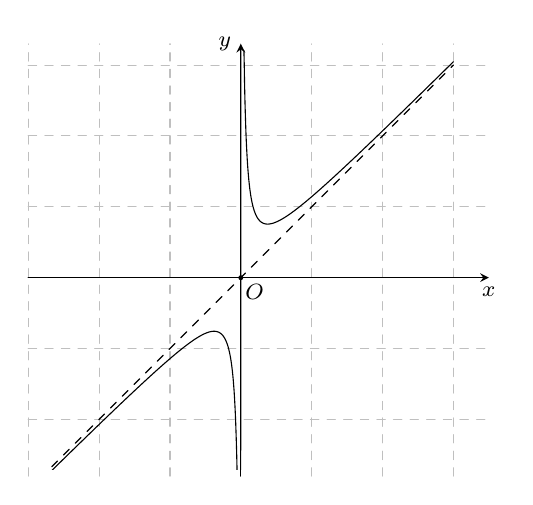
\begin{tikzpicture}[scale=.9, font=\footnotesize, line join=round, line cap=round,>=stealth]
            \def\a{0} \def\b{1} \def\c{1} \def\d{-1} % Hệ số
            \def\xmin{-3} \def\xmax{3.5}
            \def\ymin{-2.8} \def\ymax{3.3}
            \draw[color=gray!50,dashed] (\xmin,\ymin) grid (\xmax,\ymax);
            \draw[->] (\xmin,0)--(\xmax,0) node [below]{$x$};
            \draw[->] (0,\ymin)--(0,\ymax) node [left]{$y$};
            \fill (0,0) circle(1pt) node[shift=(-45:0.25)]{$O$};
            \clip (\xmin+0.1,\ymin+0.1) rectangle (\xmax-0.1,\ymax-0.1);
            \draw[smooth,samples=300,domain=-3:3] plot(\x,{\x+1/(7*\x)});
            \draw[dashed,smooth,samples=300,domain=-3:3] plot(\x,{\x});
            %	\fill (-1,0) circle (1.0pt) node[below]{$-1$} (1,0) circle (1.0pt) node[below right]{$1$};
    \end{tikzpicture}}
    \loigiai{
        \begin{itemchoice}
            \itemch $ x=0 $ là một đường tiệm cận đứng của đồ thị hàm số.
            \itemch	$ y=x $ là một đường tiệm cận xiên của đồ thị hàm số.
            \itemch $ y=x $ là một đường tiệm cận xiên của đồ thị hàm số.
            \itemch Đồ thị hàm số có $ x=0 $ là tiệm cận đứng và $ y=x $ là tiệm cận xiên nên có hai tiệm cận.
        \end{itemchoice}
    }
\end{ex}
\BTTL
\begin{ex}%[2D1K4-2]
    Nếu đồ thị hàm số $y=\dfrac{(m+1)x+2}{x-n+1}$ lần lượt nhận trục hoành và trục tung làm đường đường tiệm cận ngang và tiệm cận đứng thì $m+n$ bằng bao nhiêu?
    \shortans{$0$}
    \loigiai{
        Theo đề bài, ta có $\heva{&m+1=0\\&n-1=0} \Leftrightarrow \heva{&m=-1\\&n=1.}$\\
        Suy ra $m+n=0$.
    }
\end{ex}
\begin{ex}%[2D1K4-2]
    Tìm giá trị của $m$ để đồ thị hàm số $y=\dfrac{(2m+1)x+3}{x+1}$ có đường đường tiệm cận đi qua điểm $A(-2;7)$.
    \shortans{m=3}
    \loigiai{
        Từ đề bài, suy ra $2m+1=7 \Leftrightarrow m=3$.\\
        Suy ra $m+n=0$.
    }
\end{ex}
\begin{ex}%[2D1K4-2]
    Cho hàm số $y=\dfrac{-3+mx}{x+n}$. Tìm giá trị của $m$ và $n$ để đồ thị hàm số đã cho có tiệm cận đứng $x=2$ và tiệm cận ngang $y=2$.
    \shortans{$m=2, n=-2$}
    \loigiai{
        Từ yêu cầu đề bài, suy ra $\heva{&m=2\\&-n=2} \Leftrightarrow \heva{&m=2\\&n=-2.}$
    }
\end{ex}
\begin{ex}%[2D1K4-2]
    Để đường tiệm cận đứng và tiệm cận ngang của đồ thị hàm số $y=\dfrac{mx+1}{2m+1-x}$ cùng với hai trục tọa độ tạo thành một hình chữ nhật có diện tích bằng $3$ thì giá trị của $m$ bằng bao nhiêu?
    \shortans{$1$ hay $-\dfrac{3}{2}$}
    \loigiai{
        Từ yêu cầu đề bài, suy ra $|-m| \cdot |2m+1|=3 \Leftrightarrow \hoac{&m=1\\&m=-\dfrac{3}{2}.}$
    }
\end{ex}
\begin{ex}%[2D1K4-2]%[Thầy Hải Toán]%Câu 2.
    Đường tiệm cận đứng và đường tiệm cận ngang của đồ thị hàm số $y=\dfrac{mx+1}{2m+1-x}$ cùng với hai trục tọa độ tạo thành một hình chữ nhật có diện tích bằng $3$. Tính giá trị của $m$.
    \shortans{$m=1$; $m=-\dfrac{3}{2}$}
    \loigiai{
        Ta có $\lim\limits_{x\to+\infty}\dfrac{mx+1}{2m+1-x}=-m$; $\lim\limits_{x\to(2m+1)^+}\dfrac{mx+1}{2m+1-x} =\lim\limits_{x\to(2m+1)^+}\dfrac{m(2m+1)+1}{2m+1-x} =\lim\limits_{x\to(2m+1)^+}\dfrac{2m^2+m+1}{2m+1-x}$
        $\lim\limits_{x\to(2m+1)^+}\left(2m^2+m+1\right)=2m^2+m+1>0$; $\lim\limits_{x\to(2m+1)^+}(2m+1-x)=0$ và $2m+1-x<0\forall x>2m+1$ \\
        $ \Rightarrow\lim\limits_{x\to(2m+1)^+}\dfrac{mx+1}{2m+1-x}=-\infty $.\\
        Vậy đồ thị hàm số có hai đường tiệm cận $x=2m+1$ và $y=-m$.\\
        Hai đường tiệm cận tạo với hai trục tọa độ một hình chữ nhật có diện tích bằng $3$ suy ra $|2m+1|\cdot|m|=3\Leftrightarrow\hoac{&2m^2+m=3\\&2m^2+m=-3(PTVN)}\Leftrightarrow 2m^2+m-3=0\Leftrightarrow\hoac{&m=1\\&m=\dfrac{-3}{2}}$.}
\end{ex}
\begin{ex}%[KSCL L1, THPT Nhã Nam - Bắc Giang, 2019]%[Phạm An Bình, 12EX3]%[2D1K4-2]%
    Biết rằng đồ thị của hàm số $y=\dfrac{(n-3)x+n-2017}{x+m+3}$ ($m$, $n$ là tham số) nhận trục hoành làm tiệm cận ngang và trục tung làm tiệm cận đứng. Tính tổng $m-2n$.
    \shortans{$-9$}
    \loigiai{
        $\bullet$ $\lim\limits_{x\to +\infty}y=\lim\limits_{x\to +\infty}\dfrac{n-3+\dfrac{n-2017}{x}}{1+\dfrac{m+3}{x}} =n-3$.\\
        Vì đồ thị nhận trục hoành làm tiệm cận ngang nên $n-3=0\Leftrightarrow n=3$.\\
        $\bullet$ Vì đồ thị hàm số nhận trục tung làm tiệm cận đứng nên $\heva{&n-2017\ne 0\\&m+3=0}\Leftrightarrow \heva{&n\ne 2017\\&m= -3.}$\\
        Vậy $m-2n=-9$.
    }
\end{ex}
\begin{ex}%[TT Nguyễn Đăng Đạo, Bắc Ninh, lần 3, đề 152, 2018]%[2D1K4-2]%[Nguyễn Vân Trường, 12EX-8]%
    Tìm $m$ để tiệm cận đứng của đồ thị hàm số $y = \dfrac{m^2x-4m}{2x-m^2}$ đi qua điểm $A(2;1)$.
    \shortans{$m=-2$}
    \loigiai{
        Để hàm số có tiệm cận đứng thì \\
        $\hoac{& m \ne 0 \\ & m^2\cdot \dfrac{m^2}{2} - 4m \ne 0} \Leftrightarrow \hoac{& m \ne 0 \\ & m(m^3-8) \ne 0} \Leftrightarrow \hoac{& m \ne 0 \\ & m \ne 2}.$\\
        Khi đó tiệm cận đứng của hàm số là $x = \dfrac{m^2}{2}.$ Theo giả thiết ta có $ \dfrac{m^2}{2} = 2 \Leftrightarrow \hoac{& m =2 \text{ (loại)} \\ & m=-2 \text{ (thỏa mãn).}}$ Vậy $m=-2$.
    }
\end{ex}
\begin{ex}%[TT, Chuyên Lê Quý Đôn, Lai Châu, 2018]%[2D1K4-2]%[Nguyễn Tiến Thùy, 12EX-8]%
    Tìm $m$ để đồ thị hàm số $y=\dfrac{(m+1)x-5m}{2x-m}$ có tiệm cận ngang là đường thẳng $y=1$.
    \shortans{$m=1$}
    \loigiai{
        Ta có $\lim\limits_{x\rightarrow \pm\infty}f(x)=\lim\limits_{x\rightarrow \pm\infty}\dfrac{(m+1)x-5m}{2x-m}=\dfrac{m+1}{2}$, suy ra $y=\dfrac{m+1}{2}$ là tiệm cận ngang.\\
        Theo bài ra ta có $y=\dfrac{m+1}{2}=1\Leftrightarrow m=1$.
    }
\end{ex}
\begin{ex}%[2D1K4-1]
    Tìm tất cả các đường tiệm cận ngang của đồ thị hàm số $y=\dfrac{\sqrt{4x^2-x+1}}{2x+1}$.
    \shortans{$y=1$ và $y=-1$}
    \loigiai{
        Điều kiện xác định $x \ne \dfrac{-1}{2}$.\\
        Ta có $\lim\limits_{x \to +\infty} \dfrac{\sqrt{4x^2-x+1}}{2x+1}=\lim\limits_{x \to +\infty} \dfrac{|2x|\sqrt{1-\dfrac{1}{4x}+\dfrac{1}{4x^2}}}{2x\left(1+\dfrac{1}{2x}\right)}=1$.\\
        $\lim\limits_{x \to -\infty} \dfrac{\sqrt{4x^2-x+1}}{2x+1}=\lim\limits_{x \to -\infty} \dfrac{|2x|\sqrt{1-\dfrac{1}{4x}+\dfrac{1}{4x^2}}}{2x\left(1+\dfrac{1}{2x}\right)}=-1$.\\
        Tiệm cận ngang của đồ thị hàm số là $y= \pm 1$.
    }
\end{ex}
\begin{ex}%[2D1K4-1]
    Đồ thị hàm số $y=\dfrac{1-\sqrt{x^2+x+1}}{x^3+1}$ có tất cả bao nhiêu tiệm cận đứng và ngang?
    \shortans{$1$}
    \loigiai{
        Tập xác định $\mathscr{D}=\mathbb{R} \setminus \{-1\}$.
        \begin{itemize}
            \item
            {\allowdisplaybreaks
                \begin{eqnarray*}
                    \lim\limits_{x\to -1} \dfrac{1-\sqrt{x^2+x+1}}{x^3+1}&=&\lim\limits_{x\to -1} \dfrac{-x(x+1)}{(x+1)\left(x^2-x+1\right)\left(1+\sqrt{x^2+x+1}\right)}\\
                    &=&\lim\limits_{x\to -1} \dfrac{-x}{\left(x^2-x+1\right)\left(1+\sqrt{x^2+x+1}\right)}\\
                    &=&\dfrac{1}{6}.
            \end{eqnarray*} }
            \item $\lim\limits_{x\to +\infty}\dfrac{1-\sqrt{x^2+x+1}}{x^3+1}=0$.
        \end{itemize}
        Đồ thị hàm số không có tiệm cận đứng, tiệm cận ngang là $y=0$.
    }
\end{ex}
\begin{ex}%[2D1K4-1]
    Đồ thị hàm số $y=\dfrac{|x|}{\sqrt{x^2-1}}$ có tất cả bao nhiêu tiệm cận đứng và ngang?
    \shortans{$3$}
    \loigiai{
        Tập xác định $\mathscr{D}=(-\infty;-1) \cup (1;+\infty)$.
        \begin{itemize}
            \item $\lim\limits_{x\to-1^-}\dfrac{|x|}{\sqrt{x^2-1}}=+\infty$.
            \item $\lim\limits_{x\to 1^+}\dfrac{|x|}{\sqrt{x^2-1}}=+\infty$.
            \item $\lim\limits_{x\to +\infty}\dfrac{|x|}{\sqrt{x^2-1}}=1$.
            \item $\lim\limits_{x\to -\infty}\dfrac{|x|}{\sqrt{x^2-1}}=1$.
        \end{itemize}
        Đồ thị hàm số có $2$ tiệm cận đứng là $x=\pm 1$, tiệm cận ngang là $y=1$.
    }
\end{ex}
\begin{ex}%[2D1K4-1]
    Đồ thị hàm số $y=\dfrac{x}{\sqrt{x^2+1}}$ có tất cả bao nhiêu tiệm cận đứng và ngang?
    \shortans{$2$}
    \loigiai{
        Tập xác định $\mathscr{D}=\mathbb{R}$.
        \begin{itemize}
            \item $\lim\limits_{x\to +\infty}\dfrac{x}{\sqrt{x^2+1}}=1$.
            \item $\lim\limits_{x\to -\infty}\dfrac{x}{\sqrt{x^2+1}}=-1$.
        \end{itemize}
        Đồ thị hàm số không có tiệm cận đứng, tiệm cận ngang là $y=\pm 1$.
    }
\end{ex}
\begin{ex}%[2D1K4-1]
    Đồ thị hàm số $y=\dfrac{\sqrt{x^2-4}}{x^2-5x+6}$ có tất cả bao nhiêu tiệm cận đứng và ngang?
    \shortans{$3$}
    \loigiai{
        Tập xác định $\mathscr{D}=(-\infty;-2] \cup (2;+\infty) \setminus \{3\}$.
        \begin{itemize}
            \item $\lim\limits_{x\to 2^+}\dfrac{\sqrt{x^2-4}}{x^2-5x+6}=-\infty$.
            \item $\lim\limits_{x\to -2^-}\dfrac{\sqrt{x^2-4}}{x^2-5x+6}=-\infty$.
            \item $\lim\limits_{x\to +\infty}\dfrac{\sqrt{x^2-4}}{x^2-5x+6}=0$.
            \item $\lim\limits_{x\to -\infty}\dfrac{\sqrt{x^2-4}}{x^2-5x+6}=0$.
        \end{itemize}
        Đồ thị hàm số có $2$ tiệm cận đứng là $x=\pm 2$, tiệm cận ngang là $y=0$.
    }
\end{ex}
\begin{ex}
    Nồng độ thuốc trong máu $C(t)$ sau $t$ giờ khi uống một liều thuốc có thể được mô tả bởi hàm $C(t) = \dfrac{3}{1 + 2t}$. Tìm đường tiệm cận của nồng độ thuốc khi thời gian tăng lên rất lớn.
    \shortans{$0$}
\end{ex}
\begin{ex}
    Tốc độ (km/h) của một chiếc xe hơi tăng theo thời gian được mô tả bởi hàm $ v(t) = \dfrac{120t}{3+ t}$. Tìm đường tiệm cận của tốc độ khi thời gian tăng lên rất lớn.
    \shortans{$120$}
\end{ex}
\begin{ex}%[TeX hóa SGK CTST 12]%[Phạm Phương]%[2D1V4-4]
    Nồng độ oxygen trong hồ theo thời gian $t$ cho bởi công thức $y(t)=5-\dfrac{15t}{9t^{2}+1}$, với $y$ được tính theo mg/l và $t$ được tính theo giờ, $t \geq 0$. Tìm các đường tiệm cận của đồ thị hàm số $y(t)$. Từ đó, có nhận xét gì về nồng độ oxygen trong hồ khi thời gian $t$ trở nên rất lớn?
    \shortans{$y=5$, nồng độ tiến về $5$ mg/l}
    \loigiai{
        Hàm số $y(t)=5-\dfrac{15t}{9t^{2}+1}$ có tập xác định $\mathscr{D}=\mathbb{R}$.\\
        Ta có $\lim\limits_{x \rightarrow+\infty} \left(5-\dfrac{15t}{9t^{2}+1}\right)=5$.\\
        Vậy đồ thị hàm số có tiệm cận ngang là đường thẳng $y=5$.\\
        Khi thời gian $t$ trở nên rất lớn thì nồng độ oxygen trong hồ sẽ tiến dần về $5$ mg/l.
    }
\end{ex}
\begin{ex}
    Mô hình phát triển số lượng lợi khuẩn $P(t)$ theo thời gian có thể được mô tả bởi hàm $P(t) = \dfrac{100}{1 + 5e^{-2t}}$. Tính số lượng lợi khuẩn khi thời gian tăng lên rất lớn.\\
    \shortans{$100$}
\end{ex}
\begin{ex}
    Đáp ứng xung của một hệ thống điện tử the thời gian $t$ được mô tả bởi hàm \( h(t) = 120 e^{-\sqrt{3}t} \sin(2 t + \pi) \). Tìm và nêu ý nghĩa của đường tiệm cận của đáp ứng xung khi thời gian tăng.
    \shortans{$0$}
\end{ex}
\begin{ex}
    Điện áp của pin sạc theo thời gian được mô tả bởi hàm \( V(t) = 220 \left(1 - e^{-\dfrac{t}{\tau}}\right) \), trong đó \( \tau \) là hằng số thời gian. Tìm và nêu ý nghĩa của đường tiệm cận của điện áp khi thời gian tăng.
    \shortans{$220$}
\end{ex}
\begin{ex}%[0D1K1-4]
    Số lượng sản phẩm bán được của một công ty trong $x$ (tháng) được tính theo công thức $S(x)=200\left(5-\dfrac{9}{2+x}\right)$, trong đó $x\ge 1$ \emph{(Nguồn: R.Larson and B.Edwards, Calculus 10e, Cengage 2014).}
    \begin{enumerate}[a)]
        \item Xem $y=S(x)$ là một hàm số xác định trên nửa khoảng $[1;+\infty)$, hãy tìm tiệm cận ngang của đồ thị hàm số đó.
        \item Nêu nhận xét về số lượng sản phẩm bán được của công ty trong $x$ (tháng) khi $x$ đủ lớn.
    \end{enumerate}
    \shortans{$y=1$, sản phẩm gần $1\,000$}
    \loigiai{
        \begin{enumerate}[a)]
            \item Ta có $\lim\limits_{x\to +\infty}\left[200\left(5+\dfrac{9}{2-x}\right)\right]=200\cdot 5=1000$.\\
            Vậy $y=1\,000$ là tiệm cận ngang của đồ thị hàm số $y=S(x)$.
            \item Từ phần trên ta có thể rút ra nhận xét: khi số tháng đủ lớn thì công ty có thể bán được số sản phẩm gần bằng $1\,000$.
        \end{enumerate}
    }
\end{ex}
\begin{ex}
    Công ty cung cấp dịch vụ internet tính $75\$$ phí lắp đặt thiết bị ban đầu và phí sử dụng internet $40\$$ mỗi tháng
    \begin{listEX}
        \item Lập hàm số thể hiện chi phí sử dụng trung bình mỗi tháng sau $x$ tháng sử dụng
        \item Chi phí sử dụng trung bình thay đổi thế nào khi số tháng sử dụng tăng lên rất nhiều.
    \end{listEX}
    \shortans{$y=\dfrac{40x+75}{40}$, chi phí tiến về $40\$$}
\end{ex}
\begin{ex}
    Nhà trường dự định tổ chức tiệc liên hoan chào mừng lớp 12, tiền thuê hội trường là $1$ tỷ. Cứ mỗi người tham gia sẽ tính thêm phí phục vụ là $2$ triệu mỗi người. Gọi $x$ là số người tham gia bữa tiệc
    \begin{listEX}
        \item Lập hàm số thể hiện tổng chi phí của bữa tiệc
        \item Lập hàm số thể hiện chi phí trung bình của mỗi người bỏ ra cho bữa tiệc
        \item Chi phí trung bình của mỗi người thay đổi thế nào khi số người tham gia tăng lên rất lớn.
    \end{listEX}
    \shortans{$y=\dfrac{0,02x+1}{x}$, tiến về $2$ triệu}
\end{ex}
\begin{ex}
    Số lượng vi khuẩn trong một môi trường dinh dưỡng có thể được mô tả bởi hàm:
    \[
    N(t) = \dfrac{N_0}{1 - \dfrac{t}{T}}
    \]
    trong đó \( N(t) \) là số lượng vi khuẩn tại thời gian \( t \), \( N_0 \) là số lượng vi khuẩn ban đầu, và \( T \) là thời gian mà môi trường dinh dưỡng không còn đủ để hỗ trợ sự tăng trưởng của vi khuẩn. Xác định tiệm cận đứng của hàm số này và nêu ý nghĩa của nó.
    \shortans{$t=T$, khi $t$ tiến về $T$ thì số lượng vi khuẩn tăng lên vô hạn}
    \loigiai{
        Để tìm tiệm cận đứng, ta xem xét các giá trị của \( t \) làm cho mẫu số của phương trình bằng 0:
        \[
        1 - \frac{t}{T} = 0 \Rightarrow t = T
        \]
        Vậy đường thẳng \( t = T \) là tiệm cận đứng của đồ thị hàm số.
        \textbf{Ý nghĩa:} Từ đó ta suy ra khi thời gian \( t \) càng sát với \( T \), số lượng vi khuẩn \( N(t) \) sẽ tăng lên vô hạn. Điều này có nghĩa là khi thời gian tiếp cận \( T \) thì số lượng vi khuẩn sẽ tăng lên nhanh chóng đến mức vô hạn.}
\end{ex}
\begin{ex}
    Trong vật lý, vận tốc tối đa \(V\) của một vật rơi qua một chất lỏng được mô tả bằng phương trình:
    \[
    V(t) = \frac{mg}{b} \left(1 - e^{-\dfrac{bt}{m}}\right)
    \]
    trong đó \(m\) là khối lượng của vật, \(g\) là gia tốc trọng trường, \(b\) là hệ số ma sát, và \(t\) là thời gian. Xác định tiệm cận đứng của hàm số này và nêu ý nghĩa của nó.
    \shortans{Không có TCĐ}
    \loigiai{Để tìm tiệm cận đứng, ta xem xét các giá trị của \(t\) làm cho mẫu số của phương trình bằng 0. Tuy nhiên, trong trường hợp này, hàm số không có tiệm cận đứng vì biểu thức mũ đảm bảo hàm số được xác định cho tất cả các số thực.
        \textbf{Ý nghĩa:} Điều này ngụ ý rằng không có giới hạn về thời gian để vật đạt đến vận tốc tối đa. Khi thời gian tăng lên, vận tốc của vật sẽ tiệm cận đến vận tốc tối đa, nhưng vật không bao giờ thực sự đạt được nó.}
\end{ex}
\begin{ex}
    Trong sinh học, sự tăng trưởng của dân số \(P\) theo thời gian \(t\) có thể được mô hình bằng hàm số:
    \[
    P(t) = \frac{P_0}{1 - kP_0t}
    \]
    trong đó \(P_0\) là kích thước dân số ban đầu và \(k\) là hằng số tốc độ tăng trưởng. Xác định tiệm cận đứng của hàm số này và nêu ý nghĩa của nó.
    \shortans{$t = \frac{1}{kP_0}$}
    \loigiai{Để tìm tiệm cận đứng, ta xem xét các giá trị của \(t\) làm cho mẫu số của phương trình bằng 0:
        \[
        1 - kP_0t = 0 \Rightarrow t = \frac{1}{kP_0}
        \]
        Vậy tiệm cận đứng là \(t = \frac{1}{kP_0}\).
        \textbf{Ý nghĩa:} Điều này ngụ ý rằng hàm số tăng trưởng dân số có một tiệm cận đứng tại thời điểm \(t\) bằng nghịch đảo của tích của hằng số tốc độ tăng trưởng \(k\) và kích thước dân số ban đầu \(P_0\). Điều này chỉ ra một giới hạn cho tốc độ tăng trưởng dân số theo thời gian.}
\end{ex}
\begin{ex}
    Trong khoa học máy tính, độ phức tạp thời gian \(T(n)\) của một thuật toán với kích thước đầu vào \(n\) có thể được biểu diễn bằng hàm số:
    \[
    T(n) = \frac{an^2 + bn + c}{n}
    \]
    trong đó \(a\), \(b\), và \(c\) là các hằng số. Xác định tiệm cận đứng của hàm số này và nêu ý nghĩa của nó.
    \shortans{$T=0$}
    \loigiai{Để tìm tiệm cận đứng, ta xem xét các giá trị của \(n\) làm cho mẫu số của phương trình bằng 0:
        \[
        n = 0
        \]
        Vậy tiệm cận đứng là \(n = 0\).
        \textbf{Ý nghĩa:} Điều này ngụ ý rằng hàm số độ phức tạp thời gian không có tiệm cận đứng. Trong phân tích tính toán, một tiệm cận đứng tại \(n = 0\) sẽ ngụ ý rằng thuật toán có độ phức tạp thời gian vô hạn cho các đầu vào có kích thước bằng 0, điều này không có ý nghĩa trong hầu hết các trường hợp.}
\end{ex}
\Closesolutionfile{ans}